%%%% Proceedings format for most of ACM conferences (with the exceptions listed below) and all ICPS volumes.
\documentclass[sigconf]{acmart}
%%%% As of March 2017, [siggraph] is no longer used. Please use sigconf (above) for SIGGRAPH conferences.

%%%% Proceedings format for SIGPLAN conferences 
% \documentclass[sigplan, anonymous, review]{acmart}

%%%% Proceedings format for SIGCHI conferences
% \documentclass[sigchi, review]{acmart}

%%%% To use the SIGCHI extended abstract template, please visit
% https://www.overleaf.com/read/zzzfqvkmrfzn


%%%%%%%%%%%%%%%%%%%%%%%%%%%%%%%%%%%%%%%%%%%%%%%%%%%%%%%%%%%%%%%%%%%%%%%%%%%%%%%%%%%%%%%%%%%%%%%%%%%%%%%%%%%%%%%%%%%%%%%%%%%%%%%%%%%%%%%%%%%%%%%%%%%%%%%%%
% PACKAGES
%%%%%%%%%%%%%%%%%%%%%%%%%%%%%%%%%%%%%%%%%%%%%%%%%%%%%%%%%%%%%%%%%%%%%%%%%%%%%%%%%%%%%%%%%%%%%%%%%%%%%%%%%%%%%%%%%%%%%%%%%%%%%%%%%%%%%%%%%%%%%%%%%%%%%%%%%
\usepackage{booktabs} % For formal tables
%% perso packages:
\usepackage{epstopdf}
\usepackage{microtype}
\usepackage{tabularx}
\usepackage{multirow}
%\usepackage{arydshln}
\usepackage{subfig}
\usepackage{balance}
\usepackage{caption}
\usepackage{graphicx}

%%%%%%%%%%%%%%%%%%%%%%%%%%%%%%%%%%%%%%%%%%%%%%%%%%%%%%%%%%%%%%%%%%%%%%%%%%%%%%%%%%%%%%%%%%%%%%%%%%%%%%%%%%%%%%%%%%%%%%%%%%%%%%%%%%%%%%%%%%%%%%%%%%%%%%%%%
% DOCUMENT's Identification
%%%%%%%%%%%%%%%%%%%%%%%%%%%%%%%%%%%%%%%%%%%%%%%%%%%%%%%%%%%%%%%%%%%%%%%%%%%%%%%%%%%%%%%%%%%%%%%%%%%%%%%%%%%%%%%%%%%%%%%%%%%%%%%%%%%%%%%%%%%%%%%%%%%%%%%%%
% Copyright
%\setcopyright{none}
%\setcopyright{acmcopyright}
%\setcopyright{acmlicensed}
\setcopyright{rightsretained}
%\setcopyright{usgov}
%\setcopyright{usgovmixed}
%\setcopyright{cagov}
%\setcopyright{cagovmixed}


% DOI
\acmDOI{10.475/123_4}

% ISBN
\acmISBN{123-4567-24-567/08/06}


%%%%%%%%%%%%%%%%%%%%%%%%%%%%%%%%%%%%%%%%%%%%%%%%%%%%%%%%%%%%%%%%%%%%%%%%%%%%%%%%%%%%%%%%%%%%%%%%%%%%%%%%%%%%%%%%%%%%%%%%%%%%%%%%%%%%%%%%%%%%%%%%%%%%%%%%%
% CONFERENCE
%%%%%%%%%%%%%%%%%%%%%%%%%%%%%%%%%%%%%%%%%%%%%%%%%%%%%%%%%%%%%%%%%%%%%%%%%%%%%%%%%%%%%%%%%%%%%%%%%%%%%%%%%%%%%%%%%%%%%%%%%%%%%%%%%%%%%%%%%%%%%%%%%%%%%%%%%
%Conference
\acmConference[ICMR 2018]{ACM Yokohama conference}{June 2018}{Yokohama, Japan} 
\acmYear{2018}
\copyrightyear{2018}

\acmArticle{4}%??
\acmPrice{15.00}%??

%%%%%%%%%%%%%%%%%%%%%%%%%%%%%%%%%%%%%%%%%%%%%%%%%%%%%%%%%%%%%%%%%%%%%%%%%%%%%%%%%%%%%%%%%%%%%%%%%%%%%%%%%%%%%%%%%%%%%%%%%%%%%%%%%%%%%%%%%%%%%%%%%%%%%%%%%
\begin{document}
%%%%%%%%%%%%%%%%%%%%%%%%%%%%%%%%%%%%%%%%%%%%%%%%%%%%%%%%%%%%%%%%%%%%%%%%%%%%%%%%%%%%%%%%%%%%%%%%%%%%%%%%%%%%%%%%%%%%%%%%%%%%%%%%%%%%%%%%%%%%%%%%%%%%%%%%%

%%%%%%%%%%%%%%%%%%%%%%%%%%%%%%%%%%%%%%%%%%%%%%%%%%%%%%%%%%%%%%%%%%%%%%%%%%%%%%%%%%%%%%%%%%%%%%%%%%%%%%%%%%%%%%%%%%%%%%%%%%%%%%%%%%%%%%%%%%%%%%%%%%%%%%%%%
% TITLE
%%%%%%%%%%%%%%%%%%%%%%%%%%%%%%%%%%%%%%%%%%%%%%%%%%%%%%%%%%%%%%%%%%%%%%%%%%%%%%%%%%%%%%%%%%%%%%%%%%%%%%%%%%%%%%%%%%%%%%%%%%%%%%%%%%%%%%%%%%%%%%%%%%%%%%%%%
\title{Annotating, understanding, and predicting long-term video memorability}
\titlenote{Produces the permission block, and copyright information}
\subtitle{Extended Abstract}
\subtitlenote{The full version of the author's guide is available as
\texttt{acmart.pdf} document}

%%%%%%%%%%%%%%%%%%%%%%%%%%%%%%%%%%%%%%%%%%%%%%%%%%%%%%%%%%%%%%%%%%%%%%%%%%%%%%%%%%%%%%%%%%%%%%%%%%%%%%%%%%%%%%%%%%%%%%%%%%%%%%%%%%%%%%%%%%%%%%%%%%%%%%%%%
% AUTHORS
%%%%%%%%%%%%%%%%%%%%%%%%%%%%%%%%%%%%%%%%%%%%%%%%%%%%%%%%%%%%%%%%%%%%%%%%%%%%%%%%%%%%%%%%%%%%%%%%%%%%%%%%%%%%%%%%%%%%%%%%%%%%%%%%%%%%%%%%%%%%%%%%%%%%%%%%%
\author{Romain Cohendet}
%\authornote{}
%\orcid{1234-5678-9012}
\affiliation{%
	\institution{Technicolor}
	\streetaddress{}
	\city{Rennes} 
	\state{France} 
	\postcode{}
}
\email{romain.cohendet@technicolor.com}

\author{Karthik Yadati}
\affiliation{%
	\institution{University of Delft}
	\streetaddress{}
	\city{Delft} 
	\state{} 
	\postcode{}
}
\email{N.K.Yadati@tudelft.nl}

\author{Ngoc Khanh Duong}
\affiliation{%
	\institution{Technicolor}
	\city{Rennes} 
	\country{France}}
\email{Quang-Khanh-Ngoc.Duong@technicolor.com}

\author{Claire-Helene Demarty}
\affiliation{%
	\institution{Technicolor}
	\city{Rennes}
	\country{France}
}
\email{Claire-Helene.Demarty@technicolor.com}

% The default list of authors is too long for headers.
\renewcommand{\shortauthors}{R. Cohendet et al.}

%%%%%%%%%%%%%%%%%%%%%%%%%%%%%%%%%%%%%%%%%%%%%%%%%%%%%%%%%%%%%%%%%%%%%%%%%%%%%%%%%%%%%%%%%%%%%%%%%%%%%%%%%%%%%%%%%%%%%%%%%%%%%%%%%%%%%%%%%%%%%%%%%%%%%%%%%
% ABSTRACT
%%%%%%%%%%%%%%%%%%%%%%%%%%%%%%%%%%%%%%%%%%%%%%%%%%%%%%%%%%%%%%%%%%%%%%%%%%%%%%%%%%%%%%%%%%%%%%%%%%%%%%%%%%%%%%%%%%%%%%%%%%%%%%%%%%%%%%%%%%%%%%%%%%%%%%%%%
\begin{abstract}
Following on from the study of image memorability prediction, which draw continuous attention over the past six years, the computational understanding of video memorability's search field has recently hatched.
The growing number of shared videos foster us to find new ways to make their occurrence the most relevant in our everyday lives.
There is no available dataset of videos annotated in terms of memorability; such dataset may probably result in a launching of the field, as it had been the case for images.
The first goal of the pioneers of this search should be to succeed to propose a protocol to constitute such a dataset. 
%our work:
In this article, we propose a protocol of 700 videos annotated with memorability scores, constitute a dataset, study the quality of the collected data, and computationally modeling memorability to predict it.
%long-term memory

We finally propose a deep-learning model base to predict video memorability, comparing several methods and class of features.

\end{abstract}

%%%%%%%%%%%%%%%%%%%%%%%%%%%%%%%%%%%%%%%%%%%%%%%%%%%%%%%%%%%%%%%%%%%%%%%%%%%%%%%%%%%%%%%%%%%%%%%%%%%%%%%%%%%%%%%%%%%%%%%%%%%%%%%%%%%%%%%%%%%%%%%%%%%%%%%%%
%% NEW ACM TAXONOMY to categorise ACM article
%%%%%%%%%%%%%%%%%%%%%%%%%%%%%%%%%%%%%%%%%%%%%%%%%%%%%%%%%%%%%%%%%%%%%%%%%%%%%%%%%%%%%%%%%%%%%%%%%%%%%%%%%%%%%%%%%%%%%%%%%%%%%%%%%%%%%%%%%%%%%%%%%%%%%%%%%
\begin{CCSXML}
	<ccs2012>
	<concept>
	<concept_id>10010520.10010553.10010562</concept_id>
	<concept_desc>Computer systems organization~Embedded systems</concept_desc>
	<concept_significance>500</concept_significance>
	</concept>
	<concept>
	<concept_id>10010520.10010575.10010755</concept_id>
	<concept_desc>Computer systems organization~Redundancy</concept_desc>
	<concept_significance>300</concept_significance>
	</concept>
	<concept>
	<concept_id>10010520.10010553.10010554</concept_id>
	<concept_desc>Computer systems organization~Robotics</concept_desc>
	<concept_significance>100</concept_significance>
	</concept>
	<concept>
	<concept_id>10003033.10003083.10003095</concept_id>
	<concept_desc>Networks~Network reliability</concept_desc>
	<concept_significance>100</concept_significance>
	</concept>
	</ccs2012>  
\end{CCSXML}

%\ccsdesc[500]{Computer systems organization~Embedded systems}
%\ccsdesc[300]{Computer systems organization~Redundancy}
%\ccsdesc{Computer systems organization~Robotics}
%\ccsdesc[100]{Networks~Network reliability}

%%%%%%%%%%%%%%%%%%%%%%%%%%%%%%%%%%%%%%%%%%%%%%%%%%%%%%%%%%%%%%%%%%%%%%%%%%%%%%%%%%%%%%%%%%%%%%%%%%%%%%%%%%%%%%%%%%%%%%%%%%%%%%%%%%%%%%%%%%%%%%%%%%%%%%%%%
% KEYWORDS
%%%%%%%%%%%%%%%%%%%%%%%%%%%%%%%%%%%%%%%%%%%%%%%%%%%%%%%%%%%%%%%%%%%%%%%%%%%%%%%%%%%%%%%%%%%%%%%%%%%%%%%%%%%%%%%%%%%%%%%%%%%%%%%%%%%%%%%%%%%%%%%%%%%%%%%%%
\keywords{Video memorability, Long-term memory, Measurement protocol, Memorability scores, Deep learning, Multimedia information retrieval}

%%%%%%%%%%%%%%%%%%%%%%%%%%%%%%%%%%%%%%%%%%%%%%%%%%%%%%%%%%%%%%%%%%%%%%%%%%%%%%%%%%%%%%%%%%%%%%%%%%%%%%%%%%%%%%%%%%%%%%%%%%%%%%%%%%%%%%%%%%%%%%%%%%%%%%%%%
%% ABOUT ICMR'2018 article...
%%%%%%%%%%%%%%%%%%%%%%%%%%%%%%%%%%%%%%%%%%%%%%%%%%%%%%%%%%%%%%%%%%%%%%%%%%%%%%%%%%%%%%%%%%%%%%%%%%%%%%%%%%%%%%%%%%%%%%%%%%%%%%%%%%%%%%%%%%%%%%%%%%%%%%%%%
\maketitle
%if we want the text be called from there
 %\input{samplebody-conf}

%% About the ICMR article on Media retrieval with video memorability
	% focus on "Multimedia content-based retrieval"
	% Length: from 6 to 8 pages + 1 additional page for references (no longer distinction between long and short papers)
	% Submission deadline: 2018/01/20
	% Contributions addressing the challenges of large-scale search and user behavior analysis are especially welcome

%%%%%%%%%%%%%%%%%%%%%%%%%%%%%%%%%%%%%%%%%%%%%%%%%%%%%%%%%%%%%%%%%%%%%%%%%%%%%%%%%%%%%%%%%%%%%%%%%%%%%%%%%%%%%%%%%%%%%%%%%%%%%%%%%%%%%%%%%%%%%%%%%%%%%%%%%
\section{INTRODUCTION}%nb of sections %2 PAGES
%%%%%%%%%%%%%%%%%%%%%%%%%%%%%%%%%%%%%%%%%%%%%%%%%%%%%%%%%%%%%%%%%%%%%%%%%%%%%%%%%%%%%%%%%%%%%%%%%%%%%%%%%%%%%%%%%%%%%%%%%%%%%%%%%%%%%%%%%%%%%%%%%%%%%%%%%
%Opening
Enhancing the relevance of multimedia occurrences in our everyday life requires to imagine new ways to organize -- in particular, to retrieve -- contents.
Like other metrics of video "importance", such as aesthetics or interestingness, memorability can be regarded as a particularly relevant element to help us picking a video among several ones, with the advantage of a possibility to be measured less subjectively.

%from images to video memorability
The computational understanding of video memorability's search field follows on from the study of image memorability prediction which has attracted increasing attention from the seminal work of Isola \textit{et al.} released in 2001 \cite{isola_2011_makes}.
Recently, models of image memorability prediction achieved very good results with the introduction of deep learning to address the challenge of image memorability prediction \cite{khosla_2015_understanding,baveye_2016_deep,squalli_2017_deep}.
This success resulted on the extension of the challenge to videos.
Video memorability prediction is however a new field, and there are only two studies, to our knowledge, that addressed this issue \cite{han_2015_learning,shekhar_2017_show}.

%No dataset available
At least two important problems could explained this scarcity of studies.

%1st point: no available dataset
Firstly, there is no available dataset to train and test models.
The fact that there exist no dataset to modeling video memorability is the most serious obstacle which prevent video memorability prediction to take off.
This should be the very first goal of pioneers of this new research field: to provide data to community.
For images, the pioneers created and made downloadable such a database \cite{isola_2011_makes}, which enable to made image memorability research flourishing.
The second released database, far larger, launched new possibility for deep learning and enable to obtained the aforementioned really good results \cite{khosla_2015_understanding}.
We could expect a similar success for video memorability prediction research.
%A dataset as first objective to launch VM prediction --> Goal of this paper is to participant in the establishment of an adapted protocol
We think that the existence of such a database with high quality data could have the importance for video memorability that the ones of \cite{isola_2011_makes} and \cite{khosla_2015_understanding} had on image memorability.%in particular for deep learning algortihm which perform the best for images

%second point: difficulty to define video unity and VM
This drives us to the second point: the difficulty to build such a dataset.
The principle difficulty to define what video memorability and unity should be, and a protocol to measure items according to these definition.

If we consider the studies on image memorability prediction, we could see that, with their database, the cardinal points defined in the very first study \cite{isola_2011_makes} were widely accepted by the community without re-interrogation of what memorability -- of what the models -- really predicted.
First, it is because Isola \textit{et al.} find a proper and objective way to measure memory performance at a large scale; but it remains that how the authors proceeded is just one way to measure memorability.

From what we can imagine that such a dataset for VM will probably have an important influence on future research, one should define very carefully what memorability of video is and what the video as unity means.
It requires to define the cardinal points that will guide -- and constraint -- researchers that will used the dataset.

First, if image in image memorability was obvious, video in video memorability is less obvious.
Videos are more complex than images. Contrary to images, videos do not constitute clearly defined units, but have supplementary dimensions -- sound and movement -- that makes difficult the definition of what a video is.
%from ahn et al. Videos contain a synthesis of visual, aural, textual, and 	motion information and generally convey relatively richer 	media content than images.
By an extreme example, is it possible for a model to transfer his capacity to predict memorability from movies-like videos to Youtube-like videos?

%%%%%%%%%%%%%%%%%%%%%%
\subsection{Previous work} %Critics of the 2 previous studies
%Critics of studies on image memorability : the problem of sustainable long-term memorability
The work on image memorability prediction, initiated by \cite{isola_2011_makes}, produced great results \cite{khosla_2015_understanding,baveye_2016_deep,squalli_2017_deep}.
The availability of two large datasets \cite{isola_2011_makes,khosla_2015_understanding} has been critical in this achievement. 
However, possibly constrained by the difficulty in conducting long crowdsourcing studies, the authors measured memory performance a few minutes after memorization to obtain their memorability annotations.
As shown in \cite{cohendet_2016_prediction}, this could be a problem if we conceive that memorability reflects a lasting memory performance.
Indeed, it has long been shown that long-term memories continue to change long after their memorization through an ongoing process called consolidation \cite{mcgaugh_2000_memory}.
In particular, the early work of the psychologist Ebbinghaus showed that the drop in long-term memory performance in recall is particularly strong in the few days immediately following the memorization, after which it asymptotically tends its the almost permanent long-term performance \cite{ebbinghaus_1913_memory}.
Because several factors are susceptible to influence the consolidation process (such as the emotional content, the semantics, the attention...), which is not a linear decrease for all the memories, it follows that the order of memorability of images is susceptible to change from some minutes to a day after memorization, as it has been found in \cite{cohendet_2016_prediction} with emotional image from of the International Affective Picture System \cite{lang_2005_international}.
A protocol to collect memorability annotations for videos would benefit from the capacity to measure what we will later refer to as "long-term memorability".

%Critics of Han et al.
To our knowledge, the first attempt at predicting video memorability had been proposed by \cite{han_2015_learning}. 
The authors partially adapted the protocol proposed by \cite{isola_2011_makes} to measure image memorability for videos.
In contrast to the "memory game" proposed by Isola \textit{et al.} to collect memorability data, their protocol is however much heavier. 
They used a classical recognition task to measure memory for videos, which consists in two steps: a free viewing task, followed two days later by a recall task.
We can infer from the sparse information authors gave that the task duration, for each of the 20 participants, was about 24 hours (by taking an average video duration half-way between 15 and 30 sec), spread over 10 sessions (5 free viewing and 5 recall tasks) of about 2 hours each.
Authors used the same proportion of fillers (i.e. non repeated videos) in the free viewing and recall tasks (i.e. 4/5 of fillers and 1/5 of repeated videos named targets) to, according to them, guarantee that viewers were unaware of targets.
If it was mandatory in \cite{isola_2011_makes} for which encoding and recall tasks were interlaced, there is here a way to alleviate the task without impacting its quality; indeed, reducing the number of fillers in free viewing task would have very little impact on memorability scores (often authors even use only material interrogated later in learning/free viewing task).
Furthermore, as pointed by \cite{shekhar_2017_show}, the long time span of the experiment makes difficult the generalization of this protocol, in particular to build an extensive dataset. Regarding the prediction part, we also agree with these authors to say that the method would be difficult to generalize as it used fMRI measurements for predicting memorability.

%Critics of Shekhar et al.
Another earlier approach was the one of \cite{shekhar_2017_show}.
The participants performed a crowdsourcing experiment consisted of a free viewing task where they saw a sequences a videos, followed by a recall task for which they had to answer textual question (such as: "Did you see a man juggling?", "Did you see a car on road?").
The major drawback of the study comes from the use of questions instead of a recognition task.
Indeed, the memorability scores computed for the videos may reflect not only the differences in memory performances but also the differences between the questions in terms of difficulty, ease of understanding (in particular for the non-anglophone people that works with Amazon Mechanical Turk), of imaging, ease to retrieve a scene by some words more the by others... Especially since the authors took into account the response time of the participants to calculate the memorability scores of the videos. One will note that this potential bias could have also affect the measure of inter-human consistency.
Furthermore, the questions are handcrafted, and the choices for types of questions and videos are very limiting (e.g. the question "Did you see a car on road?" implies that in a whole experimental session you can have just one car on a road), and the authors manually ensured that no textual questions nor videos in a sequence were similar in content. This makes difficult the generalization of this protocol to build an extensive dataset.
%%% ATT!! The have tested complexity of textual questions, but there is the other problems! mesure insufisante pour rendre compte de la difficulté réelle des questions.

%%%%%%%%%%%%%%%%%%%%%%
\subsection{Goals of our study}
%Conclusion critics
It appears from the review of previous work that video memorability prediction research is in its early stage.
We still need to find a proper way to collect quality data in order to build a large dataset to bring video memorability prediction research to a new level.
%1/ we want a protocol
The present study aims to be part of these efforts to reach such a way.
As aforementioned, we also want this protocol to measure a "long-term" memorability.
This can be achieved with a study that have a long time span, where learning and recall tasks are seperated by a certain amount of time, or by measuring a memory created prior to the experiment.
Because crowdsourcing is a priori the only practicable way to experimentally collect great amount of annotations, we focused on the last choice more suitable for crowdsourcing as it requires only one connexion to the measurement application.
%2/ we want an all-around paper
To assess the quality of the data produced by the protocol, we analyzed the data obtained from different perspectives, in particular in order to shed light on some potential human or task-related factors susceptible to influence memorability as it is measured by the protocol, that are numerous \ref{cohendet_2016_using}.
%3/ we want to meet the challenge of video memorability prediction
Thanks to the data collected, we participate in the VM prediction challenge.
%Conclusion intro
The structure of the rest of the article follows these points: part 2 concerns the ground truth collection, part 3 the study of the collected data and the calculation of the memorability scores of the sequences, part 4 predicting memorability, and a conclusive part 5 where we talked about intended future work related to video memorability prediction.

%%%%%%% POTENTIALLY %%%%%%%
% Response time: must we exmploit it to calculate memorability scores?
 %Because of \cite{shekhar_2017_show} and other papers in images which suppose that short time response equal to more memorable ALORS qu'ils n'ont pas pour tâche de répondre le plus rapidement possible [vérifier].
 %La répartition du temps de réponse pourrait ne pas linéraire.
	%We hypothesized that the most memorable the sequence, the faster the participant will answer. Parce que les video les mieux représentés dans l'esprit sont les plus accessibles et que les participants ne veulent pas louper la préponse quand ils sont sûrs. % Citer papiers - s'il en existe -- où les auteurs exploitent le temps de réponse pour corriger les scores de mémorabilité;

% Personalization of the data
 %Taking into account human factors %see results Logistic regression vs. SVM

%%%%%%%%%%%%%%%%%%%%%%%%%%%%%%%%%%%%%%%%%%%%%%%%%%%%%%%%%%%%%%%%%%%%%%%%%%%%%%%%%%%%%%%%%%%%%%%%%%%%%%%%%%%%%%%%%%%%%%%%%%%%%%%%%%%%%%%%%%%%%%%%%%%%%%%%%
\section{Construction of the dataset}
%%%%%%%%%%%%%%%%%%%%%%%%%%%%%%%%%%%%%%%%%%%%%%%%%%%%%%%%%%%%%%%%%%%%%%%%%%%%%%%%%%%%%%%%%%%%%%%%%%%%%%%%%%%%%%%%%%%%%%%%%%%%%%%%%%%%%%%%%%%%%%%%%%%%%%%%%
Our first step was to implement a protocol to measure the long-term memorability of 700 video sequences, extracted from 100 mainstream movies.
The main characteristic of the protocol, in contrast with previously proposed methods to collect image and video memorability annotations, is the absence of learning/free viewing task, replaced by a questionnaire designed to collect information about the participants' prior memory.
The way of proceeding aimed at measuring memory performance after a significant retention period.

%%%%%%%%%%%%%%%%%%%%%%%%
\subsection{Dataset}
%% films and sequences
We mixed popularity and genres to establish our list of movies.% occidental movies, except for Slumdog millionaire)%to check%(list added to the appendix [ref_appendix])
Then, we manually selected seven sequences of 10 seconds from each movie (for a total of 700 sequences). %with HD or dvdrip quality, in orginal (i.e.english) version, without without subtitles [add if results HD vs. DVDrip]

%cuts
We made efforts to maintain a high intra-sequence semantic cohesion; in particular, we did not cut through meaningful vectors nor we agglomerated shots that belonged to different scenes.
Indeed, we think the images' characteristic by which they constitute obvious semantic units is an important element in the capacity of the prediction models to generalize.
By contrast, the meaning a sequence conveyed was susceptible to change depending on where we decided to cut the movie.


Because the semantics is linked to the memorability of images \cite{isola_2014_makes}, so probably to videos, therefore their memorabilities, we chose this definition susceptible to be extensive to predict other dataset.

%PARCE QUE CEST UNE PETITE BASE DE DONNEES => POUR UNE PLUS GROSSE, CE PROBLEME N4AURA PAS ROP D'EFFET.


%hence, in our idea, fostering semantics coherence of the sequences equal to diminish the difficulty of the computational models to learn without impairing their capacity to generalize.




%neutral vs. typical
We also gave preference to the sequences we called "neutral", by contrast to the "typical" ones.
According to our definition, a neutral sequence is a part of a movie which contains no element that would enable someone to easily guess it belongs to a particular movie.

The list of undesirable includes but is not limited to: recognizable famous actors, typical music, style, or any element... 

The question we asked ourselves to select the neutral sequence was the following: "Could I guess this sequence belongs to the movie I extracted it from if I didn't know it?"



In most movies, just a few or no 10-sec sequences of this sort exist. For example, in Kill Bill 1, we can 

That explains why, at the end, we obtained only 127 neutral sequences for 573 typical ones, that are defined as being non neutral sequences that meet the first criterion.


These two types of sequences -- neutral \textit{vs.} typical -- should be considered in conjunction with the instruction of the task: 

neutral sequences are control.

 of the task written above (even if you know that a sequence comes from a movie, just answer if you recognize THE sequence): 
 
They only are used as controls is just a supplementary control (qui joue un rôle symétrique au taux de FA pour la prise de risque).




%%Indoor/Outdoor
 %In Isola et al., 2014, the authors showed that memorability directly correlated with color. To explain this result, they advanced the hypothesis that the difference in memorability between indoor and outdoor scenes was due to the fact that the later tend to be less memorable that the older, and that the color tend to linked with a differences in colors, could explain this result. To validate this hypothesis, we manually annotated our 700 sequences as consisting of an indoor or outdoor scene.

%fig with video frame memorability scores ranked from most t oless memorable.




% potentially
 %First, not to be part of the official trailers, to be sure that, if a participant report not having seen the movie, he won't have seen the sequence presented for the recognition in a trailer. => Bof: this doesn't matter if False Alarms becauses of seen trailer.

%%%%%%%%%%%%%%%%%%%%%%%%
\subsection{Survey design}
%questionnaire
After they had provided basic demographics, participants filled out a questionnaire composed of 100 items, indicating whether they had seen the films of our list.
Each item included a film poster with its name below, followed by the question: "Do you remember watching (fully) this movie?" The experimenter was present in case the participant had doubt about one movie.
If the participant answered "yes", he had to answer three additional questions: "Please let us know how confident you are of having seen this movie." (I am not/slightly/50\%/considerably/100\% confident); "Please let us know when did you last see this movie." (<1 month; <1 year; <5 years; < 10 years; > 10 years); "Please let us know how many times did you watch this movie." (once; 2-4 times; 5-9 times; 10-19 times; >20 times).
If he answered "no", he had to answer one more question: "Please let us know how confident you are of NOT having seen this movie". (I am not/slightly/50\%/considerably/100\% confident).
The question relative to confidence aimed to ensure the targets and fillers corresponded to seen and non-seen films respectively.
The other questions (i.e. when and how many times the films had been seen) were used during result analysis to evaluate the likely effects of visualization repetition and passage on long-term memorability.
The questionnaire required about 20 minutes to complete.

%Algorithm selection
Based on the answers to the questionnaire, an algorithm selected 80 targets and 40 fillers among the films associated with the highest degree of certitude, with a maximum of two sequences from the same film.
Another criterion of selection for the target was the number of annotations of the sequences, in order to harmonize the nb of annotations per video.
The sequences were presented in a random order for presentation

%Recognition task
The recognition task lasted 24 minutes. Participants saw 10-seconds sequences separated by an inter-stimuli interval of 2 second. Their task was to press the spacebar when they recognized a sequence.
During the instruction, the experimenter insisted on the fact that the only task of the participant was to answer only when he recognized the particular sequence, but not answer if he recognized not even when he could guess that the sequence came from a film he had seen. This, because for number of sequences (i.e. the typical ones), it was possible to guess that the sequence came from a particular film.
Even if the participant answers, the video continue to run until its end.


%%%%%%%%%%%%%%%%%%%%%%%%
\subsubsection{Participants, facilities and apparatus}
104 participants ($22-58$ years of age; $mean = 37.1 $; $SD = 10.4 $; $26\%$ of them female), employees of [removed for double-blind review] participated in he experiment on a volunteer basis. % Technicolor, Rennes (France). All participants have either normal or corrected-to-normal visual acuity.
The videos were displayed on a ????? inch monitor (TV SONY Bravia ?????) with a display resolution of 1,920 $\times$ 1,080. The participants were seated at a distance of 150 centimeters from the screen (three times the screen height) in a room equipped with subdued lights.
%The 1,024 $\times$ 768 videos were centered on a black background; at a viewing distance of 150 cm, the stimuli subtended 18.85 degrees of vertical visual angle.

%%%%%%%%%%%%%%%%%%%%%%%%%%%%%%%%%%%%%%%%%%%%%%%%%%%%%%%%%%%%%%%%%%%%%%%%%%%%%%%%%%%%%%%%%%%%%%%%%%%%%%%%%%%%%%%%%%%%%%%%%%%%%%%%%%%%%%%%%%%%%%%%%%%%%%%%%
\section{STUDY OF THE MEMORABILITY ANNOTATIONS}
%%%%%%%%%%%%%%%%%%%%%%%%%%%%%%%%%%%%%%%%%%%%%%%%%%%%%%%%%%%%%%%%%%%%%%%%%%%%%%%%%%%%%%%%%%%%%%%%%%%%%%%%%%%%%%%%%%%%%%%%%%%%%%%%%%%%%%%%%%%%%%%%%%%%%%%%%
In this section, we analyze the ground truth data collected thanks to the protocol described in the previous section.
%%%%%%%%%%%%%%%%%%%%%%%%%%%%%%%%%%%%%
\subsection{Memorability scores calculation}
After collecting the data, we measured the average percentage of correct detections for all participants, of $46.71\%$ (SD of $14.65\%$), and the average false alarm rate, of $4.16\%$ (SD of $5.27\%$).
Then we assigned a memorability score to each sequence, defined as the percentage of correct detections by participants.
We retained only the 660 sequences that had been seen at least 4 times as targets, and remove the sequences chosen from films seen by too few participants.
On average, each sequence was viewed as target by $10.7$ participants, and as filler by $10.5$ participants.

The figure \ref{fig:overview} provides a sample of sequences sorted according to their memorability (a) and a distribution of the sequences according to their degree of memorability (b).

%Examples of ++/-- memorable sequences and Distribution of memorability scores 
\begin{figure}[!htbp]
	\centering
	\subfloat[]{\includegraphics[width=0.45\columnwidth]{figures/key_frame_mem_examples.png}}
	\quad
	\subfloat[]{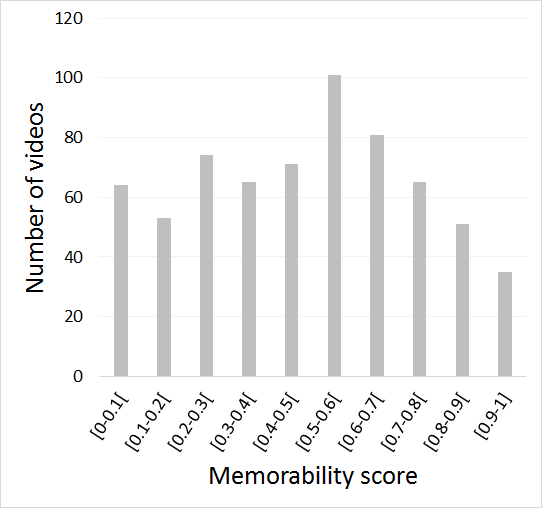
\includegraphics[width=0.45\columnwidth]{figures/memorability_scores_distribution.png}}
	\quad
	\caption{\label{fig:overview}(a) Sample of the dataset with key frames of sequences sorted from most memorable (left) to less memorable (right). (b) Distribution of the memorability scores.}
\end{figure}

%%%%%%%%%%%%%%%%%%%%%%%%%%%%%%%%%%%%%
\subsection{Consistency analysis}
%global consistency calculation
We implemented the method proposed in \cite{isola_2014_makes} to measure the human consistency.
We randomly split our 104 participants into two independent halves, and calculate how well sequence memorability scores from the first half of the participants match with sequence memorability scores from the second half of the participants.
Averaging over 25 random split half trials, we calculated a Spearman's rank correlation $\rho$ of $0.57$ between these two sets of scores.
%Individual and contextual differences, besides mandatory random variability, explain the $1-.57$ part of the memorability that is not universally derivable from the intrinsic informations of the videos.  

%Fig Consistency
%Histogram of number of nb of sequences per possibble nb of annotations
%Curve of human consistency
\begin{figure}[!htbp]
	\centering
	\subfloat[]{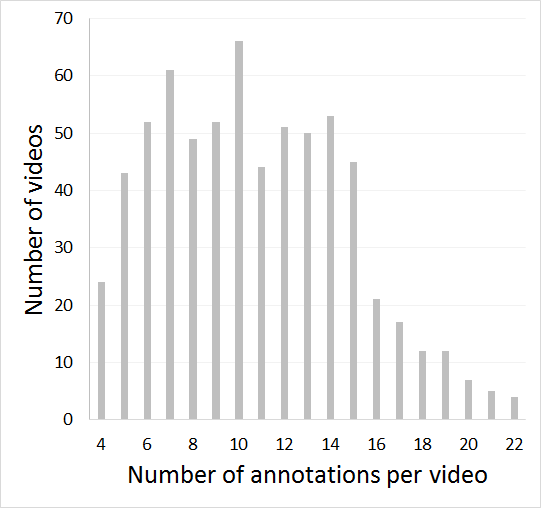
\includegraphics[width=0.45\columnwidth]{figures/histogram_nb_sequences_for_nb_of_annotations.png}}
	\quad
	\subfloat[]{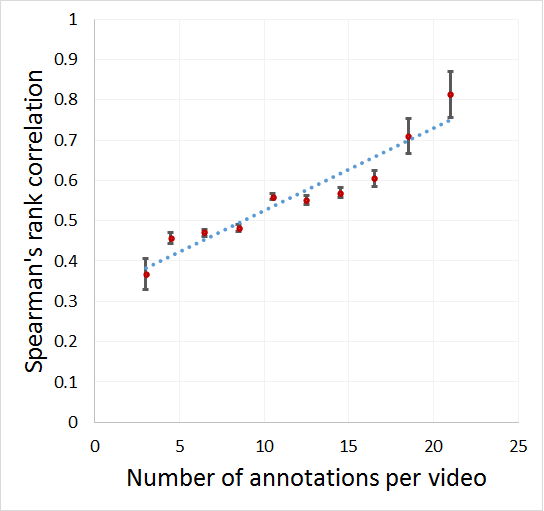
\includegraphics[width=0.45\columnwidth]{figures/Measure_of_human_consistency.png}}
	\quad
	\caption{\label{fig:human_consistency}(a) Number of sequences for each possible nb of annotations per sequence. (b) Human consistency averaged over 25 random splits (right) obtained using the method proposed by \cite{isola_2014_makes} for sequences with at least 5 annotations (with standard error and linear trendline).}
\end{figure}

%per nb of annotations consistency %comparison with image memorability
We reproduced this calculation to obtain 25 Spearman's correlation coefficients as a function of the mean number of scores per video, presented in figure \ref{fig:human_consistency}(b).
This curve is to be compared with the histogram presented in figure \ref{fig:human_consistency}(a), which shows that the number of sequences for each number of annotations was unequal.
According to the curve, we achieved a mean consistency of $.70$ around 18 annotations, which is consistent with the previous attempt of \cite{han_2015_learning}, were it is the maximum consistency they achieve.
It is interesting to compare these results to the one obtained by authors that have collected image memorability annotations \cite{isola_2011_makes,khosla_2015_understanding}.
In these studies, the authors reached such a correlation of $.70$ after 80 annotations per image, which is much later.
The experimental protocols and conditions are different between all these studies; in particular, emphasis must be placed on two points.
First, in the present studies and \cite{han_2015_learning}, we measured a long-term memory performance later than two days after the memorization, that is to say after the biggest losses in memory performance, as was previously stated. By contrast, \cite{isola_2011_makes,khosla_2015_understanding} measured memory performance from dozens of seconds to a few minutes after memorization. 
Second, videos memorability annotations were collected through in-lab experiments, and images annotations through crowdsourcing experiments.
These two confound factors may have contributed to the shortest number of annotations necessary to reach a high human consistency.
However, it would be interesting in future work to confirm if an important difference exists between images and videos regarding to the number of annotations necessary to achieve a high human response consistency.
Apart from the conclusions we could draw about the universality of the intrinsic memorability of videos compare to images, this would mean that the magnitude of the work to carry out to build an extensive database for video memorability prediction is substantially smaller than one could expect from work on image memorability prediction.

%%%%%%%%%%%%%%%%%%%%%%%%%%%%%%%%%%%%%
\subsection{Neutral and typical sequences}
% Tester s'il y a une différence entre les deux et en tirer des conséquence quant à leur validité --> How objective our measure of memorability is?
We select two sorts of sequences from the films: neutral and typical ones.
For neutral sequences, participant had no element to guess that the sequence came from a particular film; for typical sequence, participants could guess that the sequence came from a particular film.
The instructions was made clear, that we wanted that participants answered when they recognized a sequence, not when they guess that they came from a particular film they answered during the previous questionnaire film they had seen.
Thus, the response for the neutral sequences is objective, but there is subjectivity in the typical sequence.

A non-parametric Wilcoxon rank sum test showed a significant difference in memorability between the neutral ($\mu=.24$) and typical ($\mu=.53$) sequences: $Z=10.22, p<.00001$.
We expected a result in this sens because neutral sequence contained less contextual elements useful to recognize that a segment comes from a particular film.
Because of this compounding factor this results does not mean that participants tended to guess -- rather to purely recognize -- sequences drawn from films they have seen.

We also observed a difference in human consistency for memorability responses between the neutral ($\mu=.45$) and typical sequences ($\mu=.41$): $Z=2.75, p<.01$.
The human congruency was slightly higher for neutral than for typical sequences.
Along with the comments collected from the participants, who have as a majority reported difficulty to know if they guess or just recognized, this suggests that human congruence is higher for the objective measure than for a one with a part of subjectivity. In another context than with colleagues of our company, who highly probably respected the instructions -- in particular in crowdsourcing, which as we aforementioned stated that it must be used to built an extensive database -- it is probable that this difference would increase.
Certainly, this result has to be confirmed by further studies, but it could be one of the weakness of our protocol to collect extensive data.

We can also note that the false alarm rate was low for neutral sequences ($\mu=.05$) as well as for typical sequences ($\mu=.03$).
Specifically, we expect lucky confusions to account for little of correct detections on average for the two sorts of sequences.

%%%%%%%%%%%%%%%%%%%%%%%%%%%%%%%%%%%%%
\subsection{Response time}
%figure Mean response time vs. degrees of memorability
	%with SEM
\begin{figure}[!htbp]
	\centering
	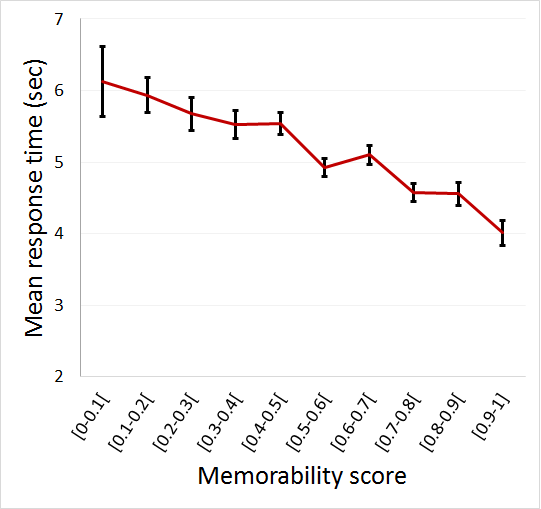
\includegraphics[width=\columnwidth]{figures/Response_time_vs_Memorability.png}
	\caption{\label{fig:response_time_vs_memorability}Mean response time for each memorability degree for targets for which participants answered(error bars correspond to SEM).}
\end{figure}

The figure \ref{fig:response_time_vs_memorability} shows that the response time to do a correct detection decreases when the memorability of the sequence increase.
We also observed a  Person's correlation of $-0.36 (p<.0001)$ between the response time on the target and their memorability scores.
These result show that the participants tended to answer quicker when the sequences were memorable than non memorable, even though the participants did not receive any instruction to answer quickly.
This suggest two things.
First, that participants tends to naturally answer rapidly after having recognized the sequence.
Second, either that the most memorable sequences are also the sequences the most accessible in memory, or that the most memorable sequences have more early recognizable elements than less memorable sequences.
However, the way we select sequences and the linear decrease in response time with memorability increasing showed in figure \ref{fig:response_time_vs_memorability} go in the direction of the first hypothesis.

%target vs. fillers
It is interesting to link it to the response time for answer on targets (i.e. correct detections) vs. on fillers (i.e. false alarms).
The global mean response time was $4.88 sec$ on targets and $5.90 sec$ on fillers.
A Wilcoxon rank sum test showed a significant difference ($Z=-5.10, p<.00001$), in the way participants globally answered more rapidly for targets (i.e. correct detections) than for fillers (i.e. false alarm).
One explanation is that participants hesitated more for fillers they answered on than to make a correct detection, increasing their response time.
This hesitation would reinforce the hypothesis that the most memorable sequences are most easily accessible in memory: if it has just been a question of a difference in the early recognizable elements that had explained that participants answered faster for the most memorable sequences, and not a question of hesitation -- i.e. of accessibility in memory --, the response time would have been the same for false alarm than for correct detection.%consistent with memory accessibility in psychology
%L’étude de la morphologie des distributions nous enseigne que le temps de réponse tend à être uniforme pour les fillers, alors que les participants répondent plus vite pour les fillers.

It also point out the fact that memories of videos are generally not obvious but more blurred.
This is an interesting point to connect with the fact that human consistency is lower for typical than for neutral sequences: because of the non obviousness of if they had memories or not, the part of subjectivity for typical sequences could have fostered participants to answer when they hesitated if they were guessing that a sequence came from a film they had seen or remembering it.
The higher degree of memorability of typical sequences compare to neutral ones could be partly due to this factor too.
Among other, this is also an argument in favour of the most "objective" possible measure to choose to constitute an extensive dataset for video memorability prediction.

To conclude this section, the degree of memorability sounds to be naturally related to response time.
Therefore, we could imagine to exploit in the calculation of memorability score.
That is what \cite{shekhar_2017_show} did in their previous attempt to construct their dataset to predict video memorability: they integrated response time in the calculation of the memorability score of their videos as the principal element (even if, in this case, the aforementioned problem of the use of questions could have influenced their results).

%%%%%%%%%%%%%%%%%%%%%%%%%%%%%%%%%%%%%
\subsection{Logistic regression vs. SVM to personalize prediction model}
%See QoMEX paper to present the data

%figure Logistic regression
\begin{figure}[!htbp]
	\centering
	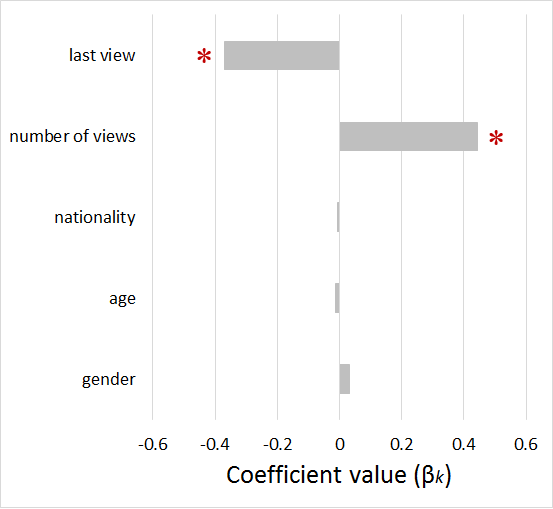
\includegraphics[width=\columnwidth]{figures/Logistic_regression.png}
	\caption{\label{fig:logistic_regression}.}
\end{figure}

%We used the following factors:
	%Occidental/non-occidental, because the 100 movies are occidental (expept slumdog millionaires...)

%Corr Evolution of the memorability along time
 %Use order positions for that (e.g. mean memorability for position 1, 2... 120)

%


%%%%%%%%%%%%%%%%%%%%%%%%%%%%%%%%%%%%%
% Other results possible
%%%%%%%%%%%%%%%%%%%%%%%%%%%%%%%%%%%%%
%\subsection{Mean memorability of the sequences compare to the film they come from}
	%Corriger score par moyenne de mem du film -- est-ce que ça a un sens ? Par le nombre de vue du film ? par le moment où il a été vu?

%\subsection{Quality of the movies}
	%dvdrip vs. HD 720-1080 => Difference of memorability? => Interesting

%\subsection{Film genre and IMDB ratings}
	%test the momorability od the sequences compare to the mean one of the movie.
	%Correct bu the mean participant's performance
	%And maybe other IMDB annotations/labels

%\subsection{Context}
	%Analyse the context (order of video presentation) influent the memo: to be check if we have enough information?
	%Une vidéo par rapport à toutes les autres différentes à un impact sur sa mem ?
	%S'inspirer de la technique de Bylinskii
	%tester la mémorability de séquences très proches (prise à intervalles très proche + vérif = même scène)

%\subsection{Features linked to memorability}
	%tester ces features comme dans 'What makes a photograph...'
	% Indoor/Outdoor, low-level visal feautures (color... -- i.e. as in isola et al.), salinecy maps

%\subsection{Indoor \textit{.vs} outdoor scenes}
	%indoor/outdoor comme isola et al. mais en contrecarrant l'effet de la couleur -- car ils expliquent que c'est par la corrrélation entre couleur et mémorabilité est expliqué par le fait que les couleurs plus froides sont d'exté.

%\subsection{Other points}
	%add other relevant points found in MIT papers e.g.


%%%%%%%%%%%%%%%%%%%%%%%%%%%%%%%%%%%%%
%\subsection{New manner to compute memorability scores: take into account time and FA}
%Une nouvelle manière pour prendre en compte les FA dans les scores de mémorabilité applicable à l'étude de la mémorabilité sur les images
%Ce qui à la fin de cette section vient avant permet de conclure cette partie en disant : la meilleure façon de calculer les scores de mémorabilité, c'est comme ça.
% The question here is: "Must we correct our memorabiliy scores by taking into account the mean memorability of the participants --> No, of the film --> No' --> So the point here is just to provide an overview.

%%%%%%%%%%%%%%%%%%%%%%%%%%%%%%%%%%%%%%%%%%%%%%%%%%%%%%%%%%%%%%%%%%%%%%%%%%%%%%%%%%%%%%%%%%%%%%%%%%%%%%%%%%%%%%%%%%%%%%%%%%%%%%%%%%%%%%%%%%%%%%%%%%%%%%%%%
\section{MEMORABILITY PREDICTION} %for Khartik
%%%%%%%%%%%%%%%%%%%%%%%%%%%%%%%%%%%%%%%%%%%%%%%%%%%%%%%%%%%%%%%%%%%%%%%%%%%%%%%%%%%%%%%%%%%%%%%%%%%%%%%%%%%%%%%%%%%%%%%%%%%%%%%%%%%%%%%%%%%%%%%%%%%%%%%%%
Until now, we have seen how we collected data and memorability annotations from users.
We then computed memorability scores and analyzed how different users fared in remembering the video sequences from the movies they have already watched.
In this section, we move towards building a machine learning model that can learn and then predict the memorability scores of a video from its audio-visual features. 
We pose the problem of predicting memorability scores as a standard regression problem and Figure \ref{prop-apprch} illustrates the different steps in our method.
From the figure, we can see that the video sequences are converted into feature vectors and then a regression model is trained that can in-turn predict the memorability scores for new video sequences.
In this following sub-sections, we explain our choice of features, models to address the problem in hand.

\begin{figure}[h]	  
  \centering
    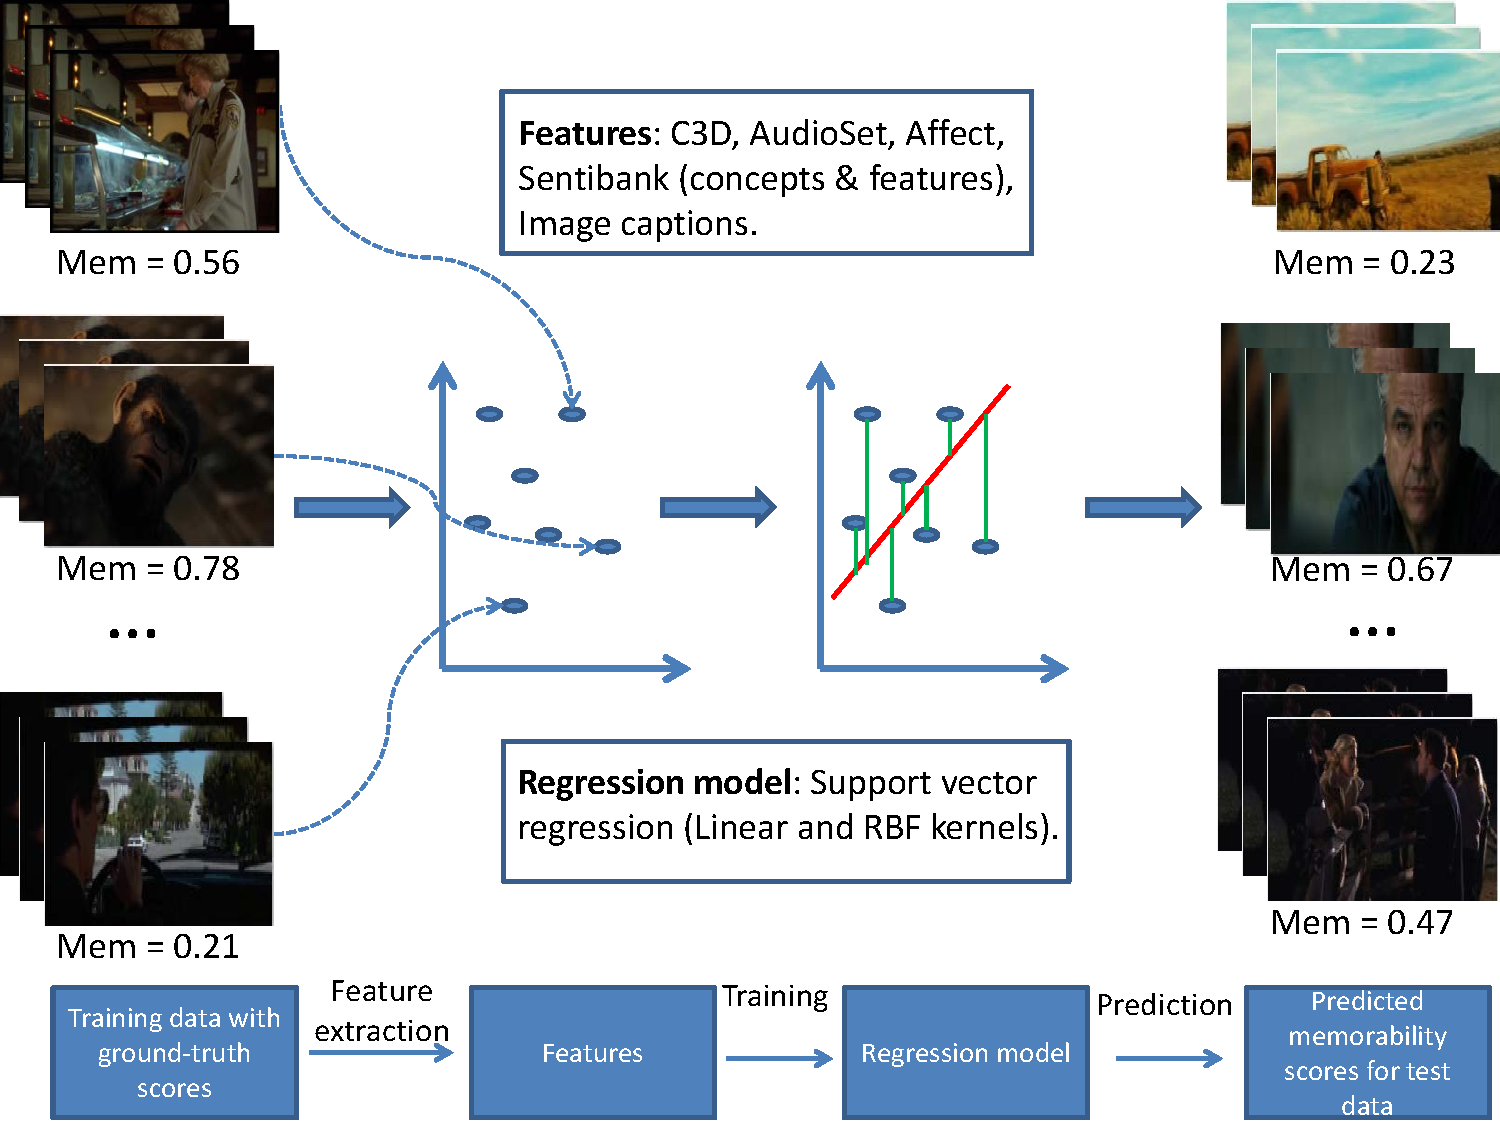
\includegraphics[width=0.9\columnwidth]{figures/approach.pdf}
		\caption{Proposed approach for automatically predicting memorability scores.}
    \label{prop-apprch}
\end{figure}

Before we go into the technical details about the different audio-visual features and regression models we explored, we will talk about how we split our dataset.
We split our dataset, at the level of movies, into training (70\%), validation (15\%) and test (15\%) data, which translates into 70 movies in the training set and 15 movies each in the validation and test sets.
We chose to split our dataset at the level of movies, instead of the video sequences, in order to avoid sequences from the same movie being present in the train as well as the evaluation set (validation+test).

\subsection{Feature extraction}
\label{feat-extr}
We explore a variety of audio-visual features in building a model that can predict memorability scores for new video sequences.
We mostly stick to state-of-the-art deep learning features that have been proposed in vision and audio research communities for tasks like video classification \cite{c3d-feat}, event detection \cite{audioset-feat}, image captioning \cite{caption-feat}, and concept detection \cite{sb-feat}. 

We use the features extracted from the C3D model, a 3-dimensional convolutional network proposed for generic video analysis \cite{c3d-feat}. 
The main motivation to use these features is that these features try to encode the motion information in the video.
The model has been proposed for video analysis and is not an extension of a model for image analysis, unlike other state-of-the-art models like VGG16 \cite{vgg16}.
We use the model trained on the Sports-1M dataset \cite{c3d-feat} that is provided by the authors of the paper.
We explore the output of the 3 fully connected layers of the network: fc6, fc7, and fc8 with a dimensionality of 4096.
Since the dimensionality of the features is very high, we also explore a dimension reduction method (Principal Component Analysis) for modelling.

Google Inc. recently released a large-scale dataset of manually annotated events: AudioSet \cite{audioset-feat}. 
The dataset consists of 10-second audio clips taken from YouTube videos along with code to extract 128-dimensional embeddings for your own audio clips.
We use these features as they are state-of-the-art in the audio event detection research and events could play a major role in how people remember sequences in movies.
We extract the 128-dimensional embeddings for our dataset and use these embeddings in training the regression models.

Now, we move onto features related to emotion.
Emotion and memory are correlated \cite{}, which is why we look at emotion related features in building a model for memorability prediction.
For emotion from visual content, we resort to a visual sentiment concept detector: Sentibank \cite{sb-feat}.
SentiBank is a set of 1200 trained visual concept detectors providing a mid-level representation of sentiment from visual content.
We use the binary code for concept detection, from images, provided by the authors.
We sample one frame for every second of the video sequence in our dataset, resulting in 10 frames per video sequence.
For each of these 10 frames, we run the sentibank concept detector and obtain two pieces of information: concepts with probabilities and features.
Concepts are adjective--noun pairs and the probability represents how likely this concept is depicted visually in that particular frame.
We rank the concepts based on the probability of their occurrence in the frame and take the top-50 concepts.
For each of the 50 concepts, we extract 300-dimensional word2vec \cite{word2vec} embeddings by training on english wikipedia corpus and taking an average of all the vectors to obtain a single vector per frame.
We repeat this process for all the 10 frames and take the average of all the vectors to obtain a single feature vector for each video.
Sentibank detectors also provide 4096-dimensional features for each frame and we take the average across all the frames to obtain one 4096-dimensional feature vector for each video.
In the end, we use two features: 300-dimensional concept vectors and 4096-dimensional feature vectors as features to build a model for memorability prediction.
Emotion will also be embedded in the audio signal and hence we resort to an audio-visual analysis of the video sequence to obtain arousal and valence scores \cite{affect}.
Arousal is the dimension of emotion that measures the excitement in the video, while valence measures whether the video happy or sad, following a circumplex model of affect \cite{affect-model}.
For each frame in the video sequence, we compute the arousal and valence scores using the methods proposed in \cite{affect}.
We concatenate the arousal and valence scores for the first 200 frames in each video sequence resulting in a 400-dimensional feature vector (200 for arousal and 200 for valence) for a video.

In addition to emotion, semantics also play a role in memory.
We utilize the ongoing research in image captioning to capture the semantics \cite{caption-feat}.
We use the code provided by the authors to extract captions for videos in our dataset.
We sample one frame for every second of the video sequence in our dataset, resulting in 10 frames per video sequence.
For each of these 10 frames, we run the caption detector and obtain a caption for the frame.
For each word in the caption, we extract 300-dimensional word2vec \cite{word2vec} embeddings by training on english wikipedia corpus and taking an average of all the words to obtain a single vector per frame.
We repeat this process for all the 10 frames and take the average of all the vectors to obtain a single feature vector for each video.
We use these 300-dimensional vectors for building our model.

\subsection{Modelling and evaluation}
\label{model-eval}
We discussed the variety of features that we extract from the audio-visual content.
Now, we turn to picking a regression model that can effectively predict memorability scores for videos in our dataset.
We choose to go with the Support vector regression model (SVR) \cite{svr}, with a linear and an RBF kernel, for its popularity and wide applicability.
Since we are posing the memorability prediction problem as a regression, we use the standard regression metric: Mean squared error ($mse$) for evaluation.
Additionally, we also use the spearmann correlation ($spcorr$) to measure the rank correlation between the predicted memorability scores and the ground-truth.
This metric gives us an indication of the correlation between the predicted memorability scores and the human annotated memorability scores.

\section{Memorability prediction results}
\label{pred-res}
In this section, we will discuss how the models trained on different features perform in predicting memorability scores of new video sequences.
Each of the video sequences in our dataset has multiple annotations and we pick sequences with atleast 4 annotations for training the models.
In our dataset, 660 sequences (need to confirm) out of the 700 sequences have atleast 4 annotations.
One set of results correspond to using these 660 sequences. 
Another set of results correspond to using 330 sequences (need to confirm) which have atleast 10 annotations. 

Since we are using an SVR with linear and rbf kernels, we train the models on the training set (70 movies) and validate the model on the validation set (15 movies).
We pick the model parameters: kernel (linear or rbf), $C$ and $\gamma$ that give the best performance in terms of $mse$ and $spcorr$.
We retrain the model with these parameters and evaluate on the final test set.
In the experiments where we use a dimension reduction method (PCA): C3D and SentiBank features, we try to retain 95\% variance in the data while reducing the feature dimensions.
Tables \ref{res-4-ann} and \ref{res-10-ann} report the memorability prediction results for different features using models trained on sequences with atleast 4 and 10 annotations.
Observing the tables, you can clearly see that the image captions perform the best among all the features.
These features capture the semantics in the video and are helping in a better prediction of the memorability scores.
The next best performance (apart from the combination of all the features) is observed for the features from the AudioSet embeddings.
Since these embeddings encode the event related information, we can say that the events happening in a video play a significant role in how the video is remembered.
A combination of all the features is the second best performing feature combination in terms of the metrics.
We concatenate all the features into a single feature vector and train a model which is then used to predict the memorability scores on the test data. 
We observe that there is a decline in performance when compared to the best performing features: image captions and this is because the other features are hindering the performance of the regression model.

One of our initial hypotheses was that emotion would play a big role in memorability of a video sequence, supported by literature from psychology.
We used different set of features to encode the emotion in a video: Affect \cite{affect} and SentiBank \cite{sb-feat}.
Observing the tables, you can say that the SentiBank features perform reasonably well, but it is not close to the performance of features encoding the semantics.
This could be because of the choice of features that encode emotion or the performance of the emotion models not being good enough for such an application.
From the analysis on this dataset and the features we used for encoding emotion, we cannot conclude that emotion plays an important role in memorability.

Comparing the results across the two tables, we observe that the model trained on sequences with atleast 4 annotations performs better than the model trained on sequences with atleast 10 annotations.
The only exception being the C3D feature, where the model trained on sequences with 10 annotations performs marginally better than the model trained on 4 annotations. 
Now, we will investigate how the performance changes with increasing number of annotations: from 4 to 15.
For this, we take the best performing feature: image captions and analyze its performance with models trained on sequences with different number of annotations.
We take sequences with 4 annotations and keep increasing the number of annotations per sequence to 15.
In each step, we repeat the training-validation-testing procedure of the previous experiment and compute the evaluation metrics.
We observed that the $mse$ does not change significantly in each of the steps and hence we provide an demonstration of how $spcorr$ varies with increasing number of annotations.
Figure \ref{num-ann} demonstrates the result of this experiment, where we observe that beyond 8 annotations the value of $spcorr$ keeps going down.

\begin{table*}[!ht]
\centering
    \begin{tabular}{| c | c | c | c |}
    \hline
				Feature& Model& $mse$& $spcorr$\\ \hline
				C3D (4096)& Linear, $C$=1.0& 0.08& 0.26\\ \hline
				C3D (PCA) (225)& Linear, $C$=1.0& 0.08& 0.21\\ \hline
				AudioSet (128)& RBF, $C$=1.0, $\gamma$=0.01& 0.06& 0.22\\ \hline
				Affect (400)& RBF, $C$=1.0, $\gamma$=0.1& 0.07& 0.17\\ \hline
				SentiBanl Conc. (300)& RBF, $C$=1.0, $\gamma$=10& 0.08& 0.13\\ \hline
				SentiBank Feat. (4096)& RBF, $C$=1.0, $\gamma$=0.1& 0.07& 0.21\\ \hline
				SentiBank Feat. (PCA) (225)& RBF, $C$=1.0, $\gamma$=0.01& 0.07& 0.21\\ \hline
				\textbf{Captions (300)}& \textbf{RBF, $C$=1.0, $\gamma$=0.01}& \textbf{0.06}& \textbf{0.31}\\ \hline
				All (1578)& RBF, $C$=1.0, $\gamma$=0.1& 0.06& 0.23\\ \hline
    \end{tabular}		
		\caption{Regression results for different features with models trained on sequences that have atleast 4 annotations.}
		\label{res-4-ann}	
\end{table*}

\begin{table*}[!ht]
\centering
    \begin{tabular}{| c | c | c | c |}
    \hline
				Feature& Model& MSE& SpearCorr\\ \hline
				C3D (4096)& Linear, $C$=1.0& 0.08& 0.24\\ \hline
				C3D (PCA) (225)& Linear, $C$=1.0& 0.09& 0.23\\ \hline
				AudioSet (128)& RBF, $C$=1.0, $\gamma$=0.1& 0.1& 0.15\\ \hline
				Affect (400)& RBF, $C$=1.0, $\gamma$=0.01& 0.09& 0.17\\ \hline
				SentiBanl Conc. (300)& Linear, $C$=1.0& 0.08& 0.14\\ \hline
				SentiBank Feat. (4096)& RBF, $C$=1.0, $\gamma$=10& 0.09& 0.14\\ \hline
				SentiBank Feat. (PCA) (225)& Linear, $C$=1.0& 0.08& 0.03\\ \hline
				\textbf{Captions (300)}& \textbf{RBF, $C$=1.0, $\gamma$=0.01}& \textbf{0.06}& \textbf{0.22}\\ \hline
				All (1578)& RBF, $C$=, $\gamma$=& 0.07& 0.21\\ \hline
    \end{tabular}		
		\caption{Regression results for different features with models trained on sequences that have atleast 10 annotations.}
		\label{res-10-ann}	
\end{table*}

\begin{figure}[h]	  
  \centering
    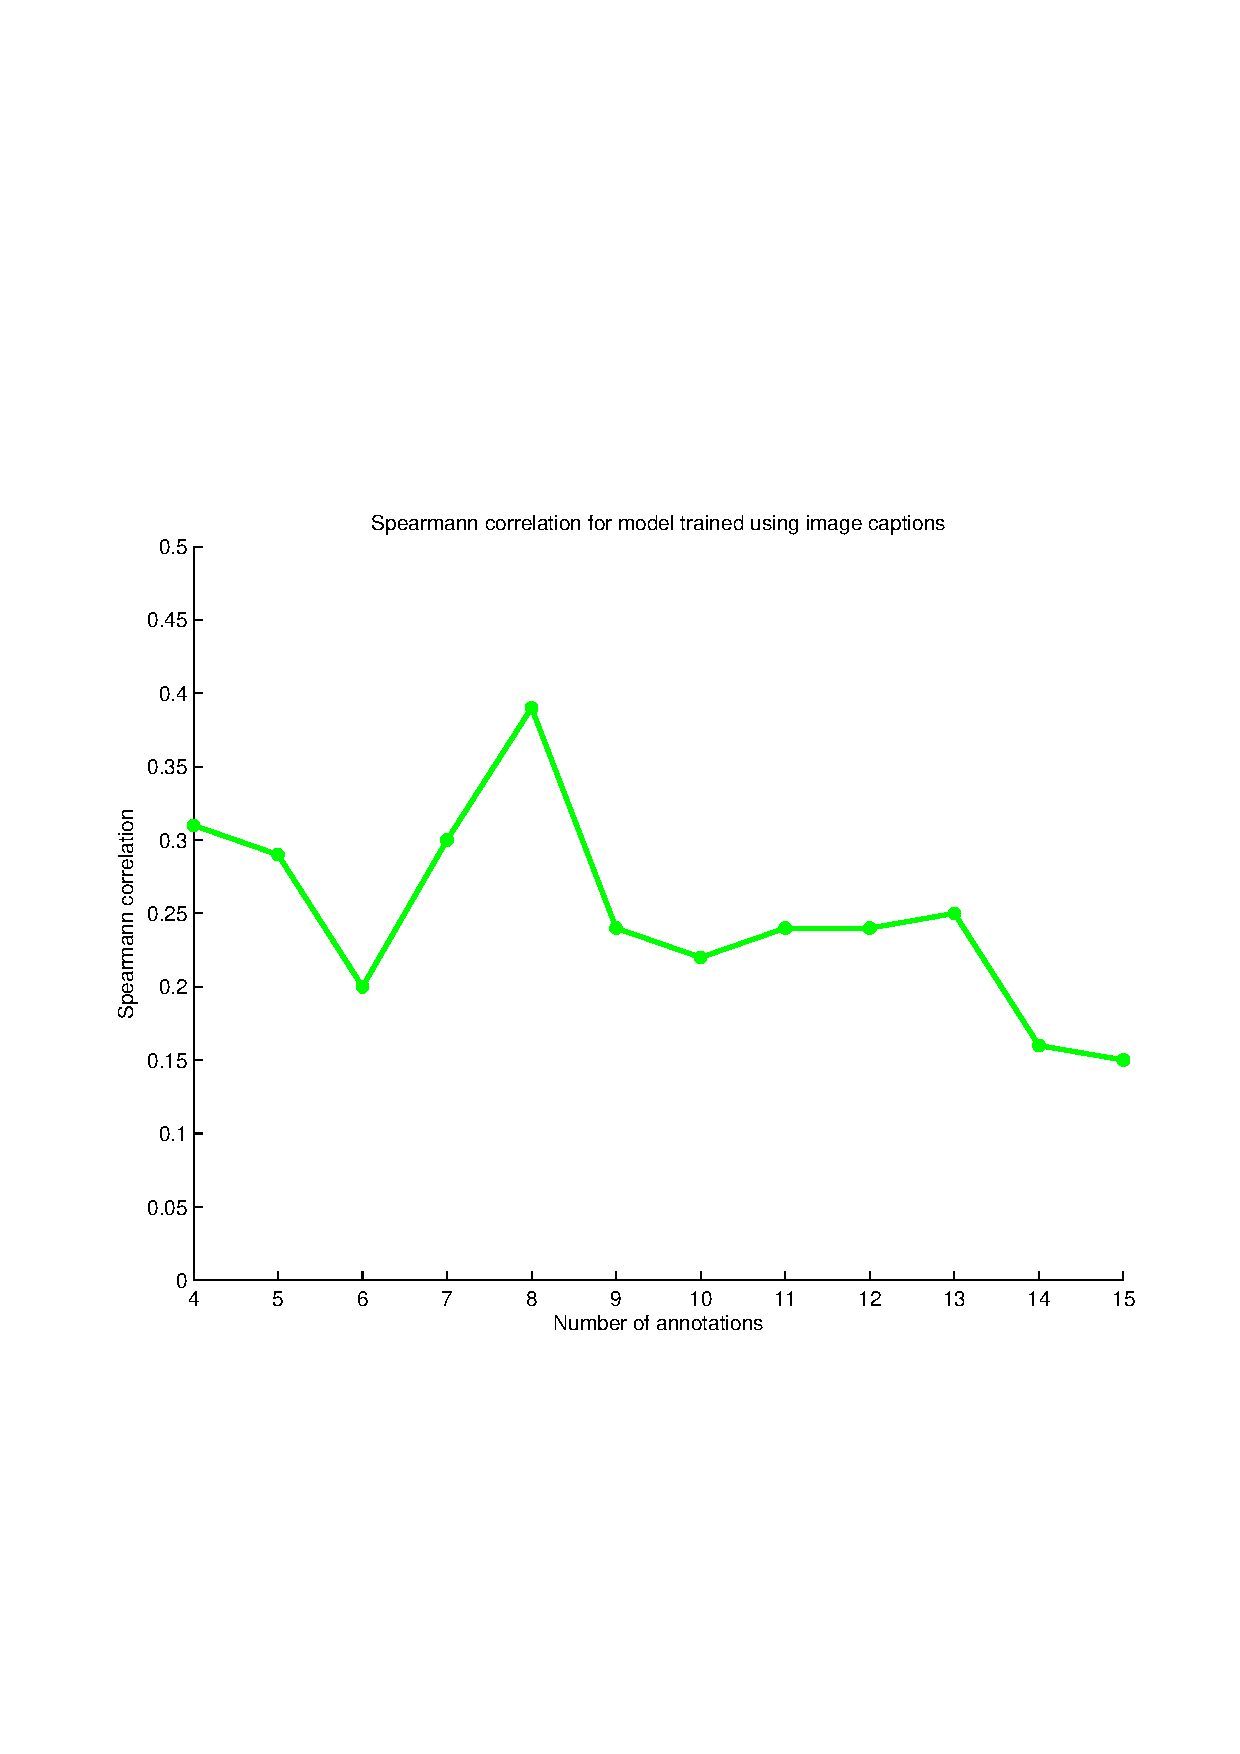
\includegraphics[width=0.7\columnwidth]{figures/annotations.pdf}
		\caption{Spearmann correlation on test data with models trained using features from image captions for varying number of annotations.}
    \label{num-ann}
\end{figure}


\subsection{Cross-validation}
\label{cross-val}
Since we have a relatively small dataset, we perform a cross-validation experiment in order to ensure that the model is not overfitting.
We perform a 10-fold cross-validation on the cross-validation set: combining the training and validation sets.
We report the results (both $mse$ and $spcorr$) of the cross-validation for the following parameters: features from image captions, model trained on sequences with atleast 4 annotations, RBF kernel.
Figure \ref{cross-val} reports the results of the cross-validation experiment and we observe that the evaluation metrics do not change much across the different folds.
We can conclude that the trained model is generalizable and there is not much overfitting.

\begin{figure}[h]	  
  \centering
    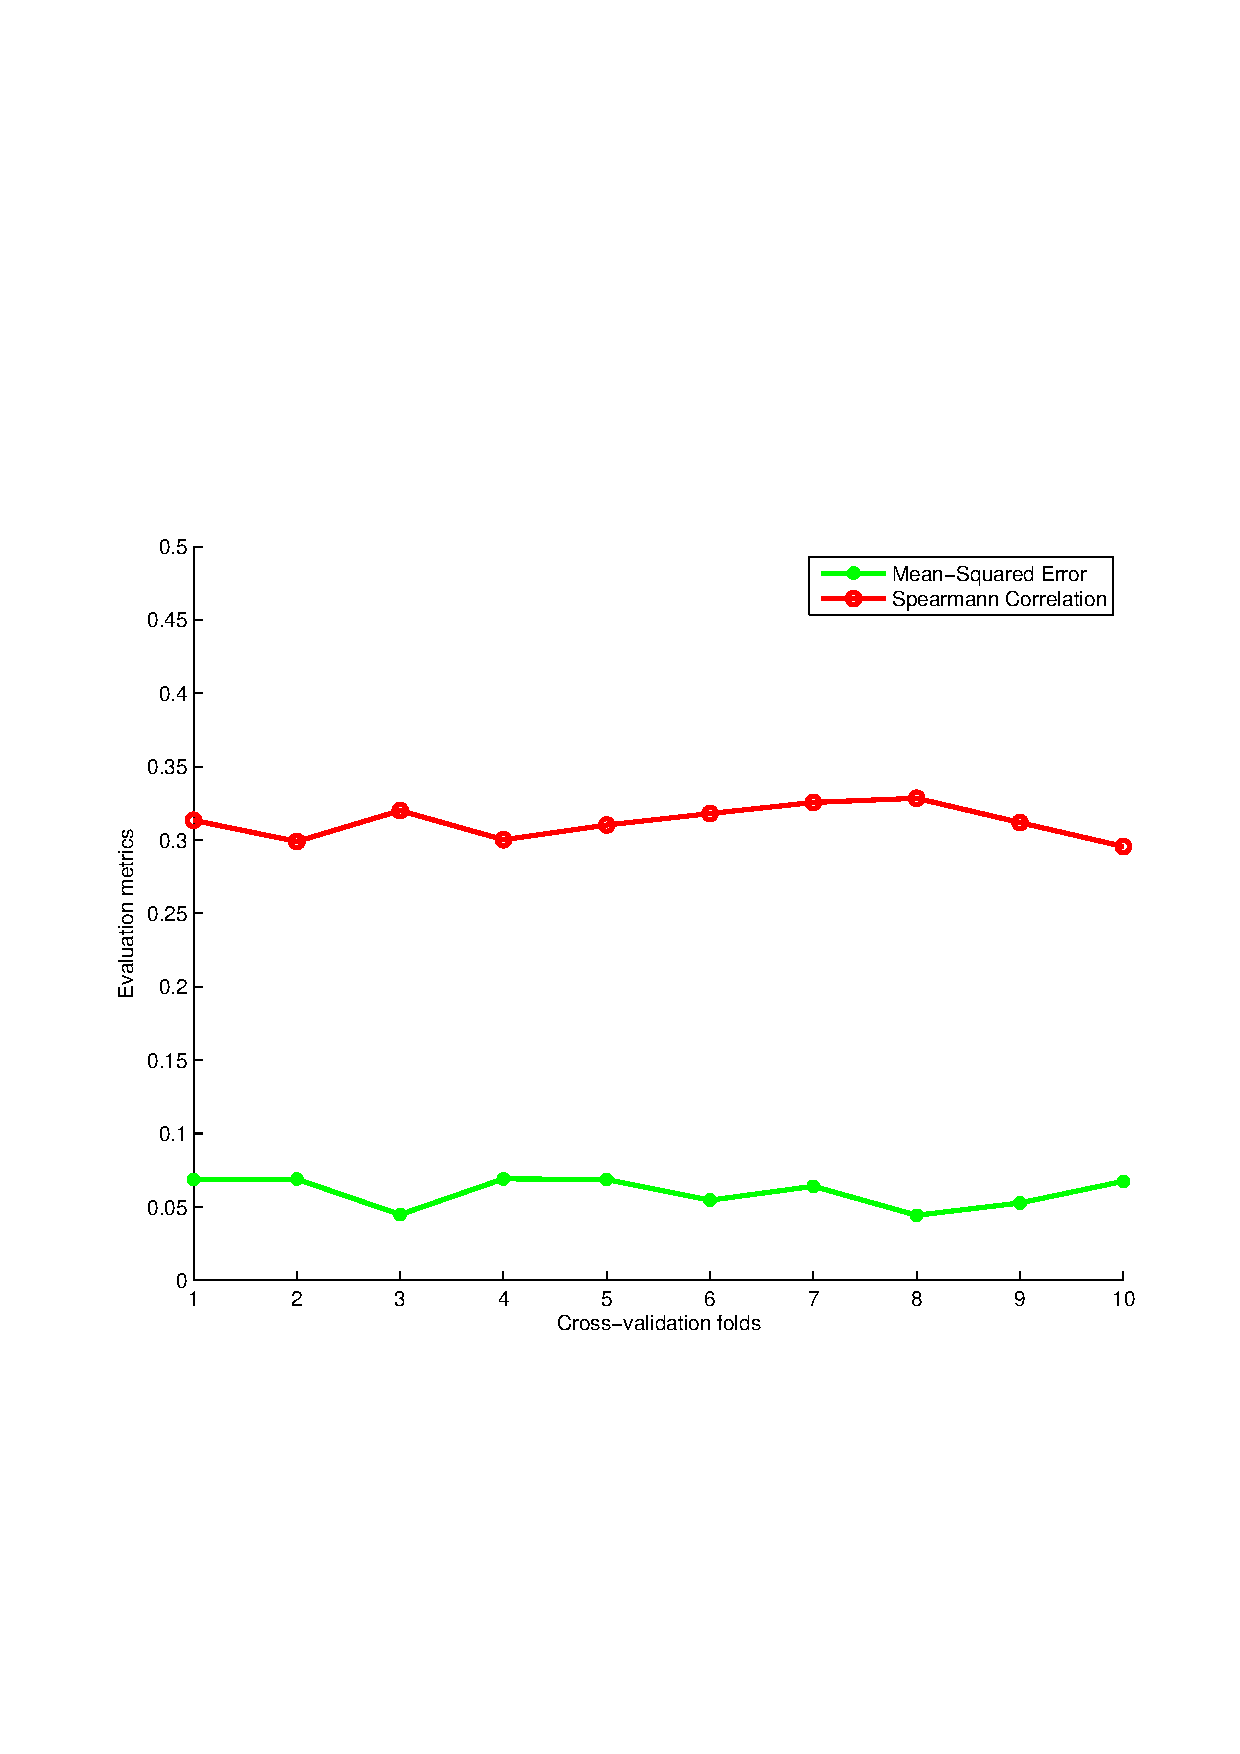
\includegraphics[width=0.8\columnwidth]{figures/cross-val.pdf}
		\caption{Cross-validation performance on a model trained on sequences with atleast 4 annotations with features from image captions and an RBF kernel.}
    \label{cross-val}
\end{figure}










%%%%%%%%%%%%%%%%%%%%%%%%%%%%%%%%%%%%%%%%%%%%%%%%%%%%%%%%%%%%%%%%%%%%%%%%%%%%%%%%%%%%%%%%%%%%%%%%%%%%%%%%%%%%%%%%%%%%%%%%%%%%%%%%%%%%%%%%%%%%%%%%%%%%%%%%%
\section{CONCLUSIONS AND FUTURE WORKS}
%%%%%%%%%%%%%%%%%%%%%%%%%%%%%%%%%%%%%%%%%%%%%%%%%%%%%%%%%%%%%%%%%%%%%%%%%%%%%%%%%%%%%%%%%%%%%%%%%%%%%%%%%%%%%%%%%%%%%%%%%%%%%%%%%%%%%%%%%%%%%%%%%%%%%%%%%
%avantages de notre dataset: long-term memorabity
%Inconvénient: mesure avec une part de subjectivité

%we propose to turn to a "totally objective" measure of memory to constitute a dataset for video memorability prediction

% Nous construisons actuellement une base de données de grande ampleur avec une mesure purement objective de la mémoire.
%Nulle part les auteurs ne parlent de mémoire à long terme, à court terme… => Ils appréhendent un problème par nature interdisciplinaire d’un point de vue purement computer science => Or la qualité des données est ce qui détermine ce que les modèles vont finalement prédire. // %D'abord, le test de mémoire interroge une mémoire de vidéos vues longtemps (en moyenne, probablement plusieurs mois ou années) auparavant.
%cite QooMEX for personlization of memorability model

% A conclusion section is not required. Although a conclusion may review the main points of the paper, do not replicate the abstract as the conclusion. A conclusion might elaborate on the importance of the work or suggest applications and extensions. 

%%%
 %Liste des features (comme/ceux de MediaEval 2015 à donner au téléchargement avec le début en sec de nos sequences)
 %Release text file for movie title, start/end time + features

%file to make the data + movies names available.

%In particular, our protocol try to correct to integrate the concept of "very long-term memory", that escaped to previous studie in image and videos, which measured the memory of items some minutes after the memory encoding.


%anntation des séquences pas à même vitesse, en cas de généralisation : changer les séquences annoté plus de 15 fois par exemple par de nouvelles.


% Conclusion => Nos travaux futurs





\addtolength{\textheight}{-12cm}   % This command serves to balance the column lengths
                                  % on the last page of the document manually. It shortens
                                  % the textheight of the last page by a suitable amount.
                                  % This command does not take effect until the next page
                                  % so it should come on the page before the last. Make
                                  % sure that you do not shorten the textheight too much.


%%%%%%%%%%%%%%%%%%%%%%%%%%%%%%%%%%%%%%%%%%%%%%%%%%%%%%%%%%%%%%%%%%%%%%%%%%%%%%%%%%%%%%%%%%%%%%%%%%%%%%%%%%%%%%%%%%%%%%%%%%%%%%%%%%%%%%%%%%%%%%%%%%%%%%%%%
\section*{APPENDIX}
%%%%%%%%%%%%%%%%%%%%%%%%%%%%%%%%%%%%%%%%%%%%%%%%%%%%%%%%%%%%%%%%%%%%%%%%%%%%%%%%%%%%%%%%%%%%%%%%%%%%%%%%%%%%%%%%%%%%%%%%%%%%%%%%%%%%%%%%%%%%%%%%%%%%%%%%%
%Appendixes should appear before the acknowledgment.

%%%%%%%%%%%%%%%%%%%%%%%%%%%%%%%%%%%%%%%%%%%%%%%%%%%%%%%%%%%%%%%%%%%%%%%%%%%%%%%%%%%%%%%%%%%%%%%%%%%%%%%%%%%%%%%%%%%%%%%%%%%%%%%%%%%%%%%%%%%%%%%%%%%%%%%%%
\section*{ACKNOWLEDGMENT}
%%%%%%%%%%%%%%%%%%%%%%%%%%%%%%%%%%%%%%%%%%%%%%%%%%%%%%%%%%%%%%%%%%%%%%%%%%%%%%%%%%%%%%%%%%%%%%%%%%%%%%%%%%%%%%%%%%%%%%%%%%%%%%%%%%%%%%%%%%%%%%%%%%%%%%%%%
%This section is optional; it is a location for you
%to acknowledge grants, funding, editing assistance and
%what have you.

%%%%%%%%%%%%%%%%%%%%%%%%%%%%%%%%%%%%%%%%%%%%%%%%%%%%%%%%%%%%%%%%%%%%%%%%%%%%%%%%%%%%%%%%%%%%%%%%%%%%%%%%%%%%%%%%%%%%%%%%%%%%%%%%%%%%%%%%%%%%%%%%%%%%%%%%%
%% BIBLIOGRAPHY
%%%%%%%%%%%%%%%%%%%%%%%%%%%%%%%%%%%%%%%%%%%%%%%%%%%%%%%%%%%%%%%%%%%%%%%%%%%%%%%%%%%%%%%%%%%%%%%%%%%%%%%%%%%%%%%%%%%%%%%%%%%%%%%%%%%%%%%%%%%%%%%%%%%%%%%%%
\bibliographystyle{ACM-Reference-Format}
\bibliography{references} 

%%%%%%%%%%%%%%%%%%%%%%%%%%%%%%%%%%%%%%%%%%%%%%%%%%%%%%%%%%%%%%%%%%%%%%%%%%%%%%%%%%%%%%%%%%%%%%%%%%%%%%%%%%%%%%%%%%%%%%%%%%%%%%%%%%%%%%%%%%%%%%%%%%%%%%%%%
\end{document}